\documentclass[tikz, border=3mm]{standalone}
\usepackage{tikz}
\usetikzlibrary{arrows.meta, decorations.markings, positioning}

\begin{document}
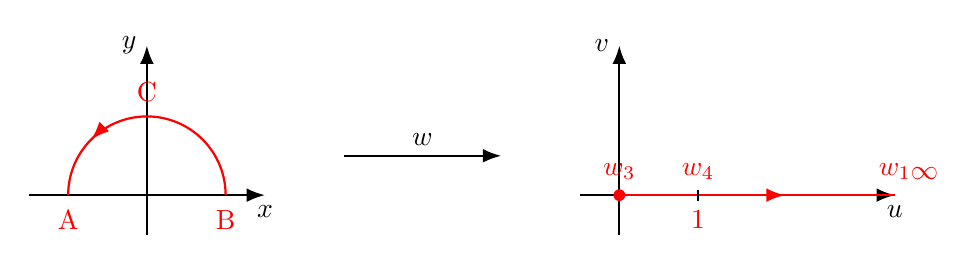
\begin{tikzpicture}[
    >=Latex, % Set default arrow tip style
    axis/.style={->, thick}, % Style for axes
    path/.style={red, thick}, % Style for the paths
    arrow/.style={decoration={markings, mark=at position #1 with {\arrow{>}}}, postaction={decorate}}, % Style for arrows on path
    arrow_rev/.style={decoration={markings, mark=at position #1 with {\arrow{<}}}, postaction={decorate}}, % Style for reversed arrows on path
    labelstyle/.style={red}, % Style for labels
    tick/.style={thick}, % Style for ticks
        red_dot/.style={fill=red, circle, inner sep=1.5pt} % Style for red point indicator
]

    % --- Left Plot (z-plane) ---
    \begin{scope}
        % Axes
        \draw[axis] (-1.5, 0) -- (1.5, 0) node[below] {$x$};
        \draw[axis] (0, -0.5) -- (0, 1.9) node[left] {$y$};

        % Define key points
        \coordinate (A) at (-1, 0);
        \coordinate (B) at (1, 0);
        \coordinate (C) at (0, 1); % Top of the arc

        % Draw arc path segment B -> A (Counter-clockwise)
        \draw[path, arrow=0.75] (B) arc (0:180:1);

        % Draw straight path segment A -> B (Commented out, as image only shows arc)
        % \draw[path, arrow=0.5] (A) -- (B);

        % Add labels for points A, B, C
        \node[labelstyle, below=2pt of A] {A};
        \node[labelstyle, below=2pt of B] {B};
        \node[labelstyle, above=2pt of C] {C};
    \end{scope}

    % --- Transformation Arrow ---
    \draw[->, thick] (2.5, 0.5) -- (4.5, 0.5) node[midway, above] {$w$};

    % --- Right Plot (w-plane) ---
    \begin{scope}[shift={(6,0)}] % Shift the second plot to the right
        % Axes
        \draw[axis] (-0.5, 0) -- (3.5, 0) node[below] {$u$};
        \draw[axis] (0, -0.5) -- (0, 1.9) node[left] {$v$};

        % Define points on u-axis
        \coordinate (w3) at (0, 0); % Origin
        \coordinate (w4) at (1, 0); % Point at u=1
        \coordinate (w1) at (3.5, 0); % Point representing infinity

        % Draw path segment w3 -> w1 with arrows indicating both directions
        \draw[path,
            arrow=0.6
            %,  % Arrow pointing right (towards w1)
           % arrow_rev=0.8 % Arrow pointing left (towards w3)
        ] (w3) -- (w1);

        % Ticks and Labels
        \draw[tick] (w3) +(0, 2pt) -- +(0, -2pt);
        \node[labelstyle, above=2pt of w3] {$w_3$};

        \draw[tick] (w4) +(0, 2pt) -- +(0, -2pt);
        \node[labelstyle, above=2pt of w4] {$w_4$};
        \node[labelstyle, below=2pt of w4] {$1$}; % Label '1' below w4

       % \draw[tick] (w1) +(0, 2pt) -- +(0, -2pt);
        \node[labelstyle, above=2pt of w1] {$w_1$};
        \node[labelstyle, above right=3pt of w1] {$\infty$}; % Infinity symbol
	 % --- Add Red Point at Origin (w3) ---
        \node[red_dot] at (w3) {};
        % --- End Red Point ---
    \end{scope}

\end{tikzpicture}
\end{document}